\documentclass[tikz,border=10pt]{standalone}
\usepackage{tikz}
\usetikzlibrary{shapes,arrows,positioning,fit,shadows}

\begin{document}
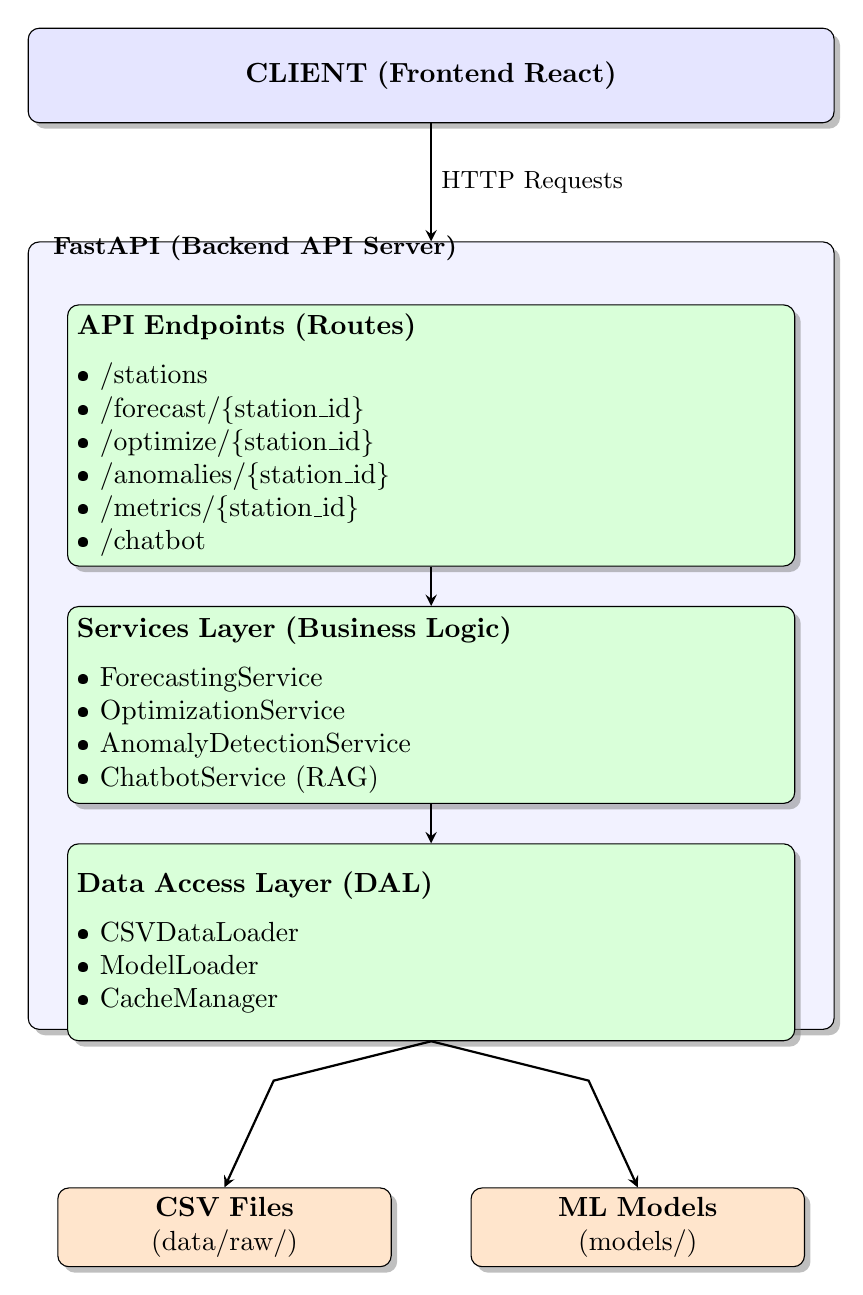
\begin{tikzpicture}[
    node distance=1cm,
    mainbox/.style={rectangle, draw, fill=blue!10, text width=10cm, minimum height=1.2cm, text centered, rounded corners, drop shadow},
    layerbox/.style={rectangle, draw, fill=green!15, text width=9cm, minimum height=2.5cm, align=left, rounded corners, drop shadow},
    databox/.style={rectangle, draw, fill=orange!20, text width=4cm, text centered, rounded corners, minimum height=1cm, drop shadow},
    arrow/.style={->, >=stealth, thick},
    label/.style={font=\small\bfseries}
]

% Client
\node[mainbox] (client) at (0,0) {
    \textbf{CLIENT (Frontend React)}
};

% FastAPI Main Box
\node[mainbox, below=1.5cm of client, minimum height=10cm, fill=blue!5] (api) {};

\node[label, above right=0.2cm and 0.2cm of api.north west, anchor=north west] {FastAPI (Backend API Server)};

% API Endpoints
\node[layerbox, below=0.8cm of api.north] (endpoints) {
    \textbf{API Endpoints (Routes)}\\[0.2cm]
    • /stations\\
    • /forecast/\{station\_id\}\\
    • /optimize/\{station\_id\}\\
    • /anomalies/\{station\_id\}\\
    • /metrics/\{station\_id\}\\
    • /chatbot
};

% Services Layer
\node[layerbox, below=0.5cm of endpoints] (services) {
    \textbf{Services Layer (Business Logic)}\\[0.2cm]
    • ForecastingService\\
    • OptimizationService\\
    • AnomalyDetectionService\\
    • ChatbotService (RAG)
};

% Data Access Layer
\node[layerbox, below=0.5cm of services] (dal) {
    \textbf{Data Access Layer (DAL)}\\[0.2cm]
    • CSVDataLoader\\
    • ModelLoader\\
    • CacheManager
};

% Data Storage
\node[databox, below left=2cm and 0.5cm of api.south] (csv) {
    \textbf{CSV Files}\\
    (data/raw/)
};

\node[databox, below right=2cm and 0.5cm of api.south] (models) {
    \textbf{ML Models}\\
    (models/)
};

% Arrows
\draw[arrow] (client.south) -- node[right, font=\small] {HTTP Requests} (api.north);
\draw[arrow] (endpoints.south) -- (services.north);
\draw[arrow] (services.south) -- (dal.north);
\draw[arrow] (dal.south) -- ++(-2,-0.5) -- (csv.north);
\draw[arrow] (dal.south) -- ++(2,-0.5) -- (models.north);

\end{tikzpicture}
\end{document}
